\indent Para verificar el correcto funcionamiento de nuestro algoritmo , elaboramos diversos tests,
los cuales ser\'an enunciados a continuaci\'on.\\

\begin{center}
 \subsubsection*{Caso 1: No existe camino para atravezar el laberinto}
\end{center}

Este caso se da cuando en cualquier camino nos encontramos con paredes irrompibles sin la posibilidad de esquivarlas.\\
 
\vspace*{0.3cm} \vspace*{0.3cm}
  \begin{center}
 %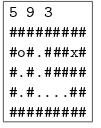
\includegraphics[scale=1.60]{./EJ1/ej1sinsolucion.jpeg}
\\{$Ejemplo$ \ 1.1 - $Caso$ $Sin$ $Soluci$\'on}
  \end{center}
  \vspace*{0.3cm}

El grafo que representa a esta entrada es de la siguiente forma:\\

\vspace*{0.3cm} \vspace*{0.3cm}
  \begin{center}
 %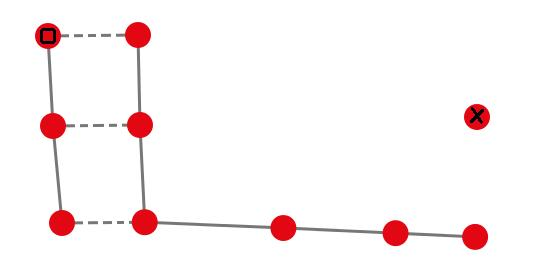
\includegraphics[scale=0.5]{./EJ1/ej1grafosinsolucion.jpeg}
 \\{$Representación$ \ 1.1 - $Caso$ $Sin$ $Soluci$\'on}
  \end{center}
  \vspace*{0.3cm}


 \begin{center}
 \subsubsection*{Caso 2: Existe un camino sin atravesar paredes para recorrer todo el laberinto}
\end{center}
 
\vspace*{0.3cm} \vspace*{0.3cm}
  \begin{center}
 %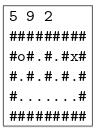
\includegraphics[scale=1.6]{./EJ1/ej1solucionsinpared.jpeg}
 \\{$Ejemplo$ \ 1.2 - $Caso$ $Sin$ $Romper$ $Paredes$}
  \end{center}
  \vspace*{0.3cm}

El grafo que representa a este tipo es de la siguiente forma:\\

\vspace*{0.3cm} \vspace*{0.3cm}
  \begin{center}
 %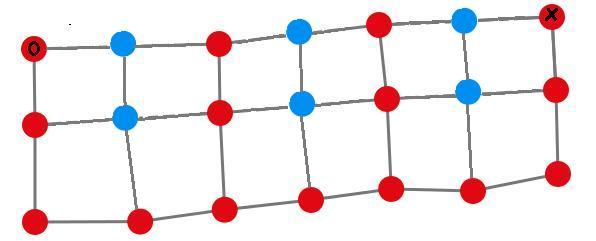
\includegraphics[scale=0.5]{./EJ1/ej1grafosolucionsinpared.jpeg}
 \\{$Representación$ \ 1.2 - $Caso$ $Sin$ $Romper$ $Paredes$}
  \end{center}
  \vspace*{0.3cm}

  
\begin{center}
 \subsubsection*{Caso 3: Rompiendo todas las paredes posibles para pasar el laberinto}
\end{center}
 
\vspace*{0.3cm} \vspace*{0.3cm}
  \begin{center}
 %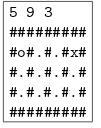
\includegraphics[scale=1.6]{./EJ1/ej1rompertodasparedes.jpeg}
\\ {$Ejemplo$ \ 1.3 - $Caso$ $Rompiendo$ $Todas$ $Paredes$ $Las$ $Posibles$}
  \end{center}
  \vspace*{0.3cm}

El grafo que representa a este tipo es de la siguiente forma:\\

\vspace*{0.3cm} \vspace*{0.3cm}
  \begin{center}
 %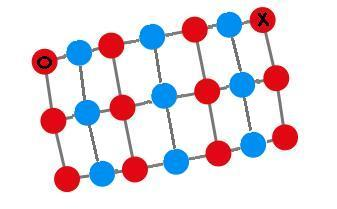
\includegraphics[scale=0.5]{./EJ1/ej1grafosolucionconpared.jpeg}
 \\{$Representación$ \ 1.3 - $Caso$ $Rompiendo$ $Todas$ $Paredes$ $Las$ $Posibles$}
  \end{center}
  \vspace*{0.3cm}


\begin{center}
  \subsubsection*{Caso 4: Rompiendo una cantidad menor de paredes posibles para pasar el laberinto}
\end{center}


\vspace*{0.3cm} \vspace*{0.3cm}
  \begin{center}
 %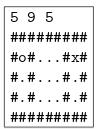
\includegraphics[scale=1.6]{./EJ1/ej1random.jpeg}
\\ {$Ejemplo$ \ 1.4 - \textit{Caso con solución}}
  \end{center}
  \vspace*{0.3cm}

El grafo que representa a este tipo es de la siguiente forma:\\

\vspace*{0.3cm} \vspace*{0.3cm}
  \begin{center}
 %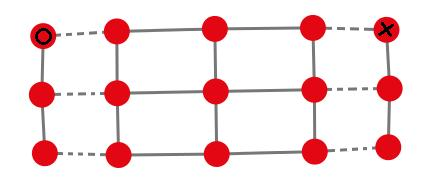
\includegraphics[scale=0.5]{./EJ1/ej1graforandom.jpeg}
 \\{$Representación$ \ 1.4 - \textit{Caso con solución}}
  \end{center}
  \vspace*{0.3cm}



\textbf{Aclaraciones:} 
\begin{itemize}
\item Nodo color celeste es una pared.
\item Nodo color rojo es caminable.
\end{itemize}
